\documentclass{ximera}
%% handout
%% nohints
%% space
%% newpage
%% numbers

%% You can put user macros here
%% However, you cannot make new environments

\graphicspath{{./}{firstExample/}{secondExample/}}

\usepackage{url}
\usepackage{tikz}
\usepackage{tkz-euclide}
\usetkzobj{all}


\tikzstyle geometryDiagrams=[ultra thick,color=blue!50!black]
\pgfplotsset{compat=1.8}
  \usepackage[T1]{fontenc}
  \usepackage[utf8x]{inputenc} %% we can turn off input when making a master document




\title{Playing With Normal Curves (Part 1)}

\begin{document}
\begin{abstract}
We will delve more deeply into the statistics of normal curves.
\end{abstract}
\maketitle

Using the link provided (\link{http://tube.geogebra.org/student/mLGTohePz}), you will find a GeoGebra App. GeoGebra is a free math program that can be used to make online interactive programs, and it can be used for a wide range of mathematical topics. At the bottom of the page, you will find three sliders, which allow you to change the values of different variables.

\begin{center}
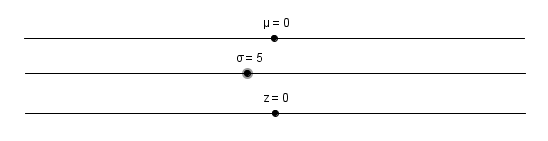
\includegraphics[scale=0.75]{Sliders.png}
\end{center}

Start with the $\mu$ slider. (The symbol $\mu$ is the Greek letter m and is read ``mu.'') You should be able to slide the dot back and forth and see the graph shift to the left and to the right. As you do this, look at the specific value of $\mu$ and you should see that it corresponds to a certain part of the graph.

\begin{question}
What phrase most accurately describes the relationship between $\mu$ and the graph?

    \begin{multipleChoice}
      \choice{As $\mu$ increases, the graph becomes squeezed together.}
      \choice[correct]{As $\mu$ increases, the graph shifts to the right.}
      \choice{As $\mu$ increases, graph becomes more spread out.}
      \choice{As $\mu$ increases, the graph shifts to the left.}
    \end{multipleChoice}

\end{question}

Set $\mu = 0$, and then play with the $\sigma$ slider. (The symbol $\sigma$ is the Greek letter s and is read ``sigma.''). 

\begin{question}
What phrase most accurately describes the relationship between $\sigma$ and the graph?

    \begin{multipleChoice}
      \choice{As $\sigma$ increases, the graph becomes squeezed together.}
      \choice{As $\sigma$ increases, the graph shifts to the right.}
      \choice[correct]{As $\sigma$ increases, graph becomes more spread out.}
      \choice{As $\sigma$ increases, the graph shifts to the left.}
    \end{multipleChoice}

\end{question}

As you continue to play with the value of $\sigma$, notice how there are four marks that change positions and change values. The values are listed above the curve at the top of the marks. You should see that the distance between those bars is equal to $\sigma$. This works regardless of the value of $\mu$. (Try it!)

Set $\mu = 0$ and $\sigma = 5$. Now play with the $z$ slider. You will notice that this doesn't change the graph, but creates a new vertical line that slides back and forth depending on the value of $z$. For example, when $z = 2.5$, the location of the vertical bar is 12.5.

Our next task will be to understand the meaning of the symbols $\mu$, $\sigma$, and $z$, and their relationship with the vertical line.

\end{document}
